%************************************************
\chapter[Axes of life history variation]{Revisiting the fast-slow continuum of 
life history variation in birds
%TODO \footnote{Submited: Maspons, J. \& D. Sol. 2021. Revisiting the fast-slow
%   continuum of life history variation in birds. \textit{????}.
%   }
}\label{ch:LHaxes}
%************************************************


\section*{Abstract}

Despite overwhelming evidence that the life history of organisms has diversified
in a broad variety of combinations of reproduction rate, age at maturity and
longevity, it is still uncertain what combinations of life history traits are
possible in nature. Here, we use an unusually large dataset of life history
information for birds to demonstrate that not all combinations of life history
traits are possible. Rather, much of life history variation is structured along
the fast-slow continuum, defined on the basis of elasticity analyses and
estimations of generation time derived from demographic models. The fast-slow
continuum may be best described by $\sim70$ (elasticity) or $\sim500$
(generation time) out of 7527 possible trait combinations, is only weakly
correlated with body mass and exhibits substantial phylogenetic signal. After
extracting the fast-slow continuum, the remaining life history variation is
structured along other less studied axes defined by the number of
reproductive bouts and the quality-quantity trade-off in egg production.
Describing the fast-slow continuum based on demographic analyses avoids the
vagueness of the concept and allows integrating it with other axes of variation,
providing a more solid basis to continue investigating the causes and
consequences of life history variation through broad comparative analyses.

\bigskip
\textbf{Keywords:} Life history, Fast-slow axis, Iteroparity, Traits' covariation

\clearpage


\section{Introduction}

Life history defines how organisms allocate their limited time and energy to
reproduction and survival \citep{stearns1992evolution}. Early works demonstrated
that the life history of organisms has diversified in an extraordinary variety
of combinations of reproduction rate, age at maturity and longevity, reflecting
the existence of trade-offs and constrains. However, it is  still uncertain
what combinations of life history traits are possible, and why some strategies
have achieved greater evolutionary success. Documenting how life history
varies across organisms is of interest in itself, and also because population
dynamics ultimately depend on how organisms allocate their limited time and
energy to reproduction and survival \citep{stearns1992evolution}. Consequently,
life history traits have a great potential to influence key ecological and
evolutionary processes, such as the likelihood of colonising new areas, the risk
of extinction and the rate of evolutionary change (see
\citet{stearns1992evolution,roff1992evolution,roff2002}).

In the last 40 years, at least 18 studies have attempted to characterize the
main axis of life history variation across species. These works use empirical
data for a set of life history traits to describe the covariation between them.
Despite the differences on the methods and taxa used all studies are consistent
on defining a “slow-fast” axis, a term first used by \citet{Stearns1983a}.
The fast-slow continuum has attracted considerable attention because it is
predicted by the age-specific mortality theory of life history evolution
\citep{Stearns1977,Charlesworth1980}⁠ and because it has implication in
understanding how organisms respond to environmental changes.

The challenge of understanding what combinations of life history traits are
possible is exemplified by the unsettled controversy about how to quantify the
fast-slow continuum axis of life history variation across species. The fast-slow
continuum aligns organisms along an axis from a “high reproductive-short life
expectancy” (fast-lived) strategy at one end to a “low reproductive-long life
expectancy” (slow-lived) strategy at the other end. Despite being one of the
most studied and influential axes of life history variation, there are notorious
discrepancies regarding how to define and quantify it across species. Indeed, at
least twelve different life history traits have been used to this purpose either
alone or in combination
often being chosen based on data availability rather than on biological
significance. For example, many studies describe the fast-slow continuum based
on surrogates of fecundity like clutch, litter size or productivity, ignoring
that a high reproductive effort has high costs in terms of survival
\citep{Adler2014}. Inconsistencies in the treatment of body size in previous
studies have also been shown to profoundly affect the quantification of the
fast-slow continuum \citep{Jeschke2009}.
Although many life history traits scale with body size, it is unclear whether
body size should be considered part of the fast-slow continuum (e.g. because
being larger improves survival) or should instead be factored out because it
merely represents constrains (e.g. it takes longer for larger organisms to
develop than it does for smaller organisms). The vagueness of the fast-slow
continuum makes the concept and its ecological and evolutionary implications
difficult to evaluate \citep{Jeschke2009}, and limits our capacity to identify
independent axes of life history variation.

The difficulties regarding how to define the fast-slow continuum across species
may come as a surprise given that early works are clear in describing it as the
result of the impossibility to simultaneously maximize survival and fecundity
\citep{Stearns1983a, Saether1988}. This means that the fast-slow continuum needs
to be understood in the context of the full lifecycle of a species. The
assessment of the relative sensitivity (i.e. elasticity) of population growth to
changes in fecundity and adult survival may be useful for this purpose, as it
helps describe the fecundity-survival trade-off. Thus, a slow-lived strategy
should be characterised by high elasticities to the adult survival and low
elasticities to fecundity, the contrary being true for fast-lived species.
According to \citet{Gaillard1989}, the fast-slow continuum can also be 
represented as a time scale gradient ranking species according to turnover (see 
also \citet{Jeschke2009,Saether2013,Adler2014}⁠). Under this view, the
fast-slow should be better characterised by estimating generation time, where a 
long generation time is a distinctive feature of slow-lived strategies.

While demographically-derived approaches to the fast-slow continuum represent
important advances, resulting in metrics that are more accurate and
demographically meaningful, the paucity of information of species’ life cycles
limits their application to broad comparative analyses that are geographically
and taxonomically representative. This severely limits our capacity to discern
what combinations of life history traits are possible in nature. One way to
overcome such a limitation is to use a demographically-derived approach to
identify the combinations of life history traits that best predict either
generation time or the fecundity-survival trade-off (i.e. elasticities to
fecundity and adult survival), and then use the best combinations to estimate
the position in the fast-slow continuum of species for which information of the
full life cycle is not available.

In the present paper, we use this framework to characterise the fast-slow
continuum of birds, a group that has played a pivotal role in developing life
history theory but for which characterizing the fast-slow continuum has proved
particularly difficult. We first estimate elasticities to the adult survival and
generation time for a subset of species for which demographic data are
available. We then explore the extent to which all the combinations of the 14
life history traits most commonly used to describe the fast-slow continuum 
predict variation in elasticities and generation time. Once the best 
combinations of traits are identified, we use them to classify 
\textgreater{1000} species along the fast-slow continuum.

We finally investigate the life history variation that remains once variation
in the fast-slow continuum is factored out, and describe three extra axes
related to iteroparity, development time, and the quality-quantity trade-off for
the offspring.


\section{Methods}

\subsection*{Life history traits}

We assembled published information on the 14 life history traits most often used
to describe the fast-slow continuum (Table \ref{tab:table2.1}). These traits
describe adult quality (LFS, RLS, AFB), juvenile quality (DP, I, FLE, EMR,
OV), the investment in offspring (FEC, CS, PRO, PEP), iteroparity (BV), and body
mass (BM). We found information of the 14 life history traits for 
\textgreater{6700} species (full life history dataset; see Table 
\ref{tab:table2.1} for details), and complete information for 797 species 
(restricted life history dataset). All traits were log-transformed except BV, 
OV and EMR.


\begin{table}
\caption[Life history traits]{Life history traits considered in the present
study. Sample size is the number of species for which information is
available.}\label{tab:table2.1}
\begin{tabular}{@{}p{2.5cm}cp{7.5cm}p{1.5cm}@{}}
\toprule
Trait                         & Abbreviation & Definition                                   & Sample size \\
\midrule
Maximum lifespan              & LFS          & Maximum recorded lifespan                    & 1583        \\
Maximum reproductive lifespan & RLS          & LFS - AFB                                    & 1088        \\
Age at first breeding         & AFB          & Age at which individuals start reproducing   & 1205        \\
Developmental period          & DP           & Period from egg laying to fledging (I + FLE) & 1907        \\
Incubation                    & I            & Period from egg laying to hatching           & 2577        \\
Fledging                      & FLE          & Period from hatching until fledging          & 1980        \\
Egg mass residual             & EMR          & Relative egg mass                            & 4074        \\
Fecundity                     & FEC          & $CS$ multiplied by the number of broods per year         & 1633 \\
Clutch size                   & CS           & Number of eggs in a given clutch             & 6551 \\
Productivity                  & PRO          & Egg mass * fecundity / body mass             & 1582 \\
Potential Egg Production      & PEP          & $PRO * RLS$                                  & 901 \\
Brood value                   & BV           & $log10\left(\tfrac{1}{ broods \cdot RLS } \right)$       & 909  \\
Offspring value               & OV           & $log10\left(\tfrac{1}{ FEC \cdot RLS } \right)$          & 909 \\
Body mass                     & BM           & Weight                                       & 6462        \\
\bottomrule
\end{tabular}
\end{table}

\subsection*{Restrictions in the life history traits space}

With our life history dataset, we first investigated which portion of the 
dimensional trait space is occupied by birds that nowadays live on Earth. We 
restricted this analysis to 9 life history traits (LFS, EMR, BM, DP, FLE, 
AFB, CS, FEC, BV), to avoid redundancies and to reduce the computational cost, 
and used them to compute a nine-dimensional convex hull volume containing 95\% 
of the observed combinations of the traits. The volume of the hull 
was compared with mean hypervolumes generated from 4 null models randomised 
999 times ($Hv_{nm}$ hereafter), following \citet{Diaz2016}⁠.
Hypervolumes in $Hv_{nm1}$ to $Hv_{nm3}$ assume that the traits vary
independently. Null model 1 assumes that any combination of trait values can 
exist with equal probability, each trait having a uniform distribution 
approximating an hypercube. Null model 2 assumes that extreme trait values are 
selected against during evolution and each trait has a normal distribution, 
with $Hv_{nm2}$ approximating an hypersphere. Null model 3 imposes no
assumptions about trait distributions but instead allows each trait to be
distributed as observed and assumes traits are independent of each other. Null
model 4 assumes that extreme values are selected against (i.e., normally
distributed) and maintains the observed correlation structure among traits.
Relative to null models 1 to 3, null model 4 collapses the multidimensional
trait-space occupied by birds ($Hv_{nm4}$) into an elongated hyperellipsoid.


\subsection*{Identifying the life history traits that best describe the 
fast-slow continuum}

We used the COMADRE Matrix Database Version 4.20.11.0 
\citep{Salguero-Gomez2016} to obtain age-structured population models that 
incorporate accurate information on the rates of survival, growth, and 
reproduction for 174 bird populations belonging to 78 species (demographic 
dataset, hereafter). For each species we selected population matrices from 
wild, unmanipulated populations with complete data instead of pooled from 
different populations if available (n = 42). See figure \ref{fig:fig2.1} to 
compare the distribution of the life history traits using the restricted 
dataset and the subset with demographic data from the population matrices.

\begin{figure}
\centering
\includegraphics[width=\textwidth]{./Figures/chapter02/fig1-LH_demo_traits.png}
\caption[Traits distribution]{
Biplots (upper triangle) and density plots (lower triangle) of the traits. 
Black for species with either demographic or traits data and red dots for 
species with both demographic (gen.T for generation time and elas.A for 
elasticities to the adult survival) and life history traits data (see table
\ref{tab:table2.1} for details).}
\label{fig:fig2.1}
\end{figure}

From each population matrix model, we calculated 2 demographic 
traits \citep{Caswell2001,Stubben2007}: generation time and elasticity to the
adult survival. The elasticity matrices show the proportional effects on 
population growth rate for each demographic trait \citep{deKroon2000}⁠. We 
selected elasticities to the adult survival and net fecundity as a measure of
the importance of these components on the life history strategies. However, both
elasticities were perfectly correlated (correlation coefficient = 1) and we only 
used the elasticities to the adult survival.

To assess how well life history traits correlate with the estimated demographic 
traits, we used the 14 life history traits previously described (Table 
\ref{tab:table2.1}), which were available for the 30 species. The estimated 
elasticities and generation times were modelled as a function of life history 
traits by means of phylogenetic least square regressions (with Pagel’s 
$\lambda$ estimated by means of maximum likelihood), as implemented in the R 
package “phylolm” \citep{Ho2014}⁠. The traits were tested alone and combined 
with other traits by means of phylogenetic principal component analysis 
(PPCA), with maximum likelihood estimates of $\lambda$, as implemented in 
“phytools” \citep{Revell2009a}⁠. The phylogenetic analyses were run with 
2 consensus trees from \citet{Jetz2012}, one for the Ericsson and 
one for the Hackett backbones.
The PPCAs were obtained using the restricted life history dataset (n = 797). We 
assembled all combinations of traits with the only rule that a PPCA should 
include at least a trait related to adult quality, juvenile quality and the 
number of offspring. A total of 10080 combinations of traits were used in the 
PPCAs, from which 2464 were discarded due to unsatisfactory convergence, 
resulting in 7616 trait combinations with a proper PPCA. For each PPCA, we 
selected the Principal Component (PC) that better match the demographic traits 
($\Delta AIC = 0$) and flipped the axis when 
needed, multiplying the PC scores and loadings by -1 in order to sort the 
species from fast (negative values) to slow (positive values).

From all the studied traits, whether alone or combined in a PC, we 
considered those that better explain variation in elasticities or generation 
time as corresponding to the fast-slow axis. We tested their relative 
importance by estimating the AIC based weight of each regression, considering 
the best models as those with 2 units difference from the model with the lowest 
AIC ($\Delta AIC < 2$).


\subsection*{Defining species position on the fast-slow axes}

Our previous analyses are based on the combination of detailed demographic data 
and full life history information for 30 species. If there are combinations of 
life history traits that accurately predicts variation in elasticities and/or 
generation time, it is possible to use the life history information to assess 
the position in the fast-slow continuum for species for which demographic data 
was unavailable. We defined the position of the species in the fast-slow axis 
as the mean scores of the PCs weighted by the AIC based weights 
of the elasticity models (FSe) and generation time models (FSgt). We did the 
same using all selected PCs and using only the PCs of the best models only 
($\Delta AIC < 2$).

Our finding that to accurately predict elasticities and/or generation time you 
only need a few life history traits, not all of them, open the possibility to 
assess the position in the fast-slow continuum for many more species than those 
with full information on the 14 key life history traits. Therefore, we repeated 
each of the PPCAs identified as best predictors of elasticities and generation 
time in the previous analyses, but now including all the species for which 
information on the underlying life history traits was available, regardless that 
other traits were missing. As before, we defined their position as the mean 
scores of best PCs weighted by the AIC based weights of the elasticity 
and generation time models (FSe and FSgt).

Our extrapolations to estimate the fast-slow axes assumes that the studied
subsets of species are representative of the observed variation in the fast-slow
continuum.
This assumption is supported by two analyses. First, the phylogenetically 
corrected correlation \citep{Revell2009a}⁠ of the relevant PCs estimated with
the demographic, restricted and full life history datasets was
\textgreater{0.99} in all cases.
Second, the mean values of each PC estimated for our subsets of species (i.e.
the demographic and restricted datasets) do not significantly differ from those
expected by randomly sampling the same number of species from the full life
history dataset.


\subsection*{Other axes of life history variation}

We analysed the remaining ~9500 (from 9385 to 9604 depending on the life 
history dataset and phylogeny) significant PCs (eigenvalue \textgreater{1}) not 
selected as components of the fast-slow axes to explore potentially different
axes of variation. First, we used the correlation among the scores of the PCs to
build clusters using different minimum absolute correlations (0.7 – 0.9),
discarding clusters containing less than 5\% of the PCs and removing duplicated
clusters in different correlation thresholds.
For each group, we flip the PCs to align the scores and loadings when needed. 
Every cluster represents a potential axis of life history variation. We grouped 
clusters with a correlation on averaged loadings \textgreater{0.95} for 
visualization purposes.


\subsection*{Characterisation of the life history axes}

For each potential axis, we calculated the mean and the standard deviation of 
the loadings and the relative frequency of the traits for the included PPCAs,
assuming that the loadings of missing traits in a PPCA is 0. As the frequencies
of the traits were not the same for each cluster, we also estimated the
relative weight of each trait as:
% the proportion of the absolute values of the loadings in a PC minus the
% relative frequency of the traits in the PC cluster:
$$ Relative~weight = \frac{ \left \lvert L \right \rvert } { \sum{\left \lvert L \right \rvert} } - \frac{ Freq } { \sum{Freq} } $$
% Lmat = matrix(loadings, cols=LHT, rows=PCA)
%
% # Missing traits = 0 Loading
%  Loads<- colSums(Lmat / nrow(Lmat), na.rm=TRUE)
%
%  Freq<- colSums((!is.na(Lmat))  / nrow(Lmat), na.rm=TRUE)
%
% # sum(Freq.prop) == 1
%  Freq.prop<- Freq / sum(Freq)
%
% # sum(traitsLw.weight.prop) == 1
%  Lw.weight.prop<- abs(Loads) / sum(abs(Loads))
%  diff.weight<- Lw.weight.prop -  Freq.prop
Where $L$ is a vector with the mean loadings of each trait and $Freq$ is a
vector with the number of PPCAs from the cluster that contain the trait. The
relative weight of the traits ranges from -1 to 1, where negative values means
that the absolute value of the trait loadings are lower than expected by the
frequency of the trait and positive values for traits with higher loadings than
expected by the frequency of the trait. For the fast-slow axes we weighted the
former metrics by the AIC based weight from all the models and also including
only the best models.

For each defined axis, we averaged the scores of the species to generate a data 
base of life history for birds. Again, for the fast-slow axes we weighted the
PCs scores by the AIC based weight for all models and also using the PCs in the
best models only. The averaged scores of the fast-slow axes where then used to
predict elasticities to the adult survival and generation time to compare the
performance against the scores of single PCs.


\section{Results}

The observed hypervolume based on the 9 non-redundant life history traits is 
much smaller than the hypervolumes predicted by the null models (p-value = 
0.001, see table \ref{tab:table2.2}). The closest null model, $Hv_{nm4}$, is
the one that imposes a correlation among traits as observed but still 7 times 
larger than the hypervolume of the observed data. The smaller size and 
aggregation in the hypervolume indicate that not all trait combinations are 
possible, consistent with the existence of constrains and trade-offs in the life 
history evolution. The observed aggregation of species is greater for the 
observed traits than the expected for each $Hv_{nm}$ (table
\ref{tab:table2.2}). Thus, the existing diversity of life history strategies 
seems restricted to certain combinations of correlated traits and shows a 
greater concentration in the trait space than expected under multivariate 
normality.

\begin{table}
\center
\caption[Species' concentration and hypervolumes]{The world's bird species are
concentrated in nine-trait space as compared to expectations under theoretical
null models and fills a much more restricted hypervolume. Minimum number of 
cells within nine-trait multivariate space (divided in $10^{6}$ cells) needed to
cover 10\% (N10) or 50\% (N50) of species in the observed hypervolume 
($Hv_{obs}$) and in four different null-model simulated hypervolumes 
($Hv_{nm1-4}$) and the volume of each hypervolume (the mean of the 999 
permutations for $Hv_{nm}$). See main text for details.}
\label{tab:table2.2}
\begin{tabular}[b]{@{}lccc@{}}
\toprule
\textbf{Hypervolume} & \textbf{N10} & \textbf{N50} & \textbf{Volume} \\
\midrule
$Hv_{obs}$  & 9   & 71  & 4.3 \\
$Hv_{nm1}$  & 131 & 354 & 1030450 \\
$Hv_{nm2}$  & 131 & 397 & 10808.4 \\
$Hv_{nm3}$  & 131 & 394 & 8187 \\
$Hv_{nm4}$  & 131 & 312 & 30.6 \\
\bottomrule
\end{tabular}
\end{table}

From the 7631 trait combinations, including single traits, the selected PCs 
scores from the PPCAs combining sets of traits, and other metrics used to 
describe the fast-slow continuum in the literature, 104 where among 
the ones that better predict elasticities to the adult survival
($\Delta AIC < 2$), while for predicting generation time 468 trait combinations
where among the bests. All the best predictors are PCs scores except for the
single trait clutch size that is also part of the best predictors for the
elasticity to the adult survival.
The best PCs come from PPCA with $5.9 \pm 1.3$ combined traits for adult 
survival elasticities and $6.2 \pm 1.3$ for generation time. The adjusted $R^2$
of the PCs explain $55\% \pm 0.008$ of the elasticities to the adult survival
and $48\% \pm 0.008$ for generation time. Here we report the results for the
restricted life history dataset using the phylogeny based on the Hackett
backbone and the best PCs only ($\Delta AIC < 2$). See table
\ref{tab:tabApp2.1} for the details of the extended life history dataset (maxN)
and the models with the phylogeny based on the Ericson backbone.

Although single traits are often used as surrogate for the fast-slow axis, only
CL appears among the best models for elasticity to the adult survival ($\Delta
AIC = 0.6$ ) and no single trait for generation time (see
\href{https://github.com/jmaspons/Thesis/tree/master/ESM/chapter02}{
FS\_modelSelection.xlsx in the ESM}). The ratio FEC / AFB, which has also been
suggested to accurately describe the fast-slow axis \citep{Oli2004}⁠, is not
among the best traits, alone or in combination, that better explains adult
survival elasticities ($\Delta$AIC = 85.6) nor generation time ($\Delta$AIC =
10.2).

\begin{figure}
\centering
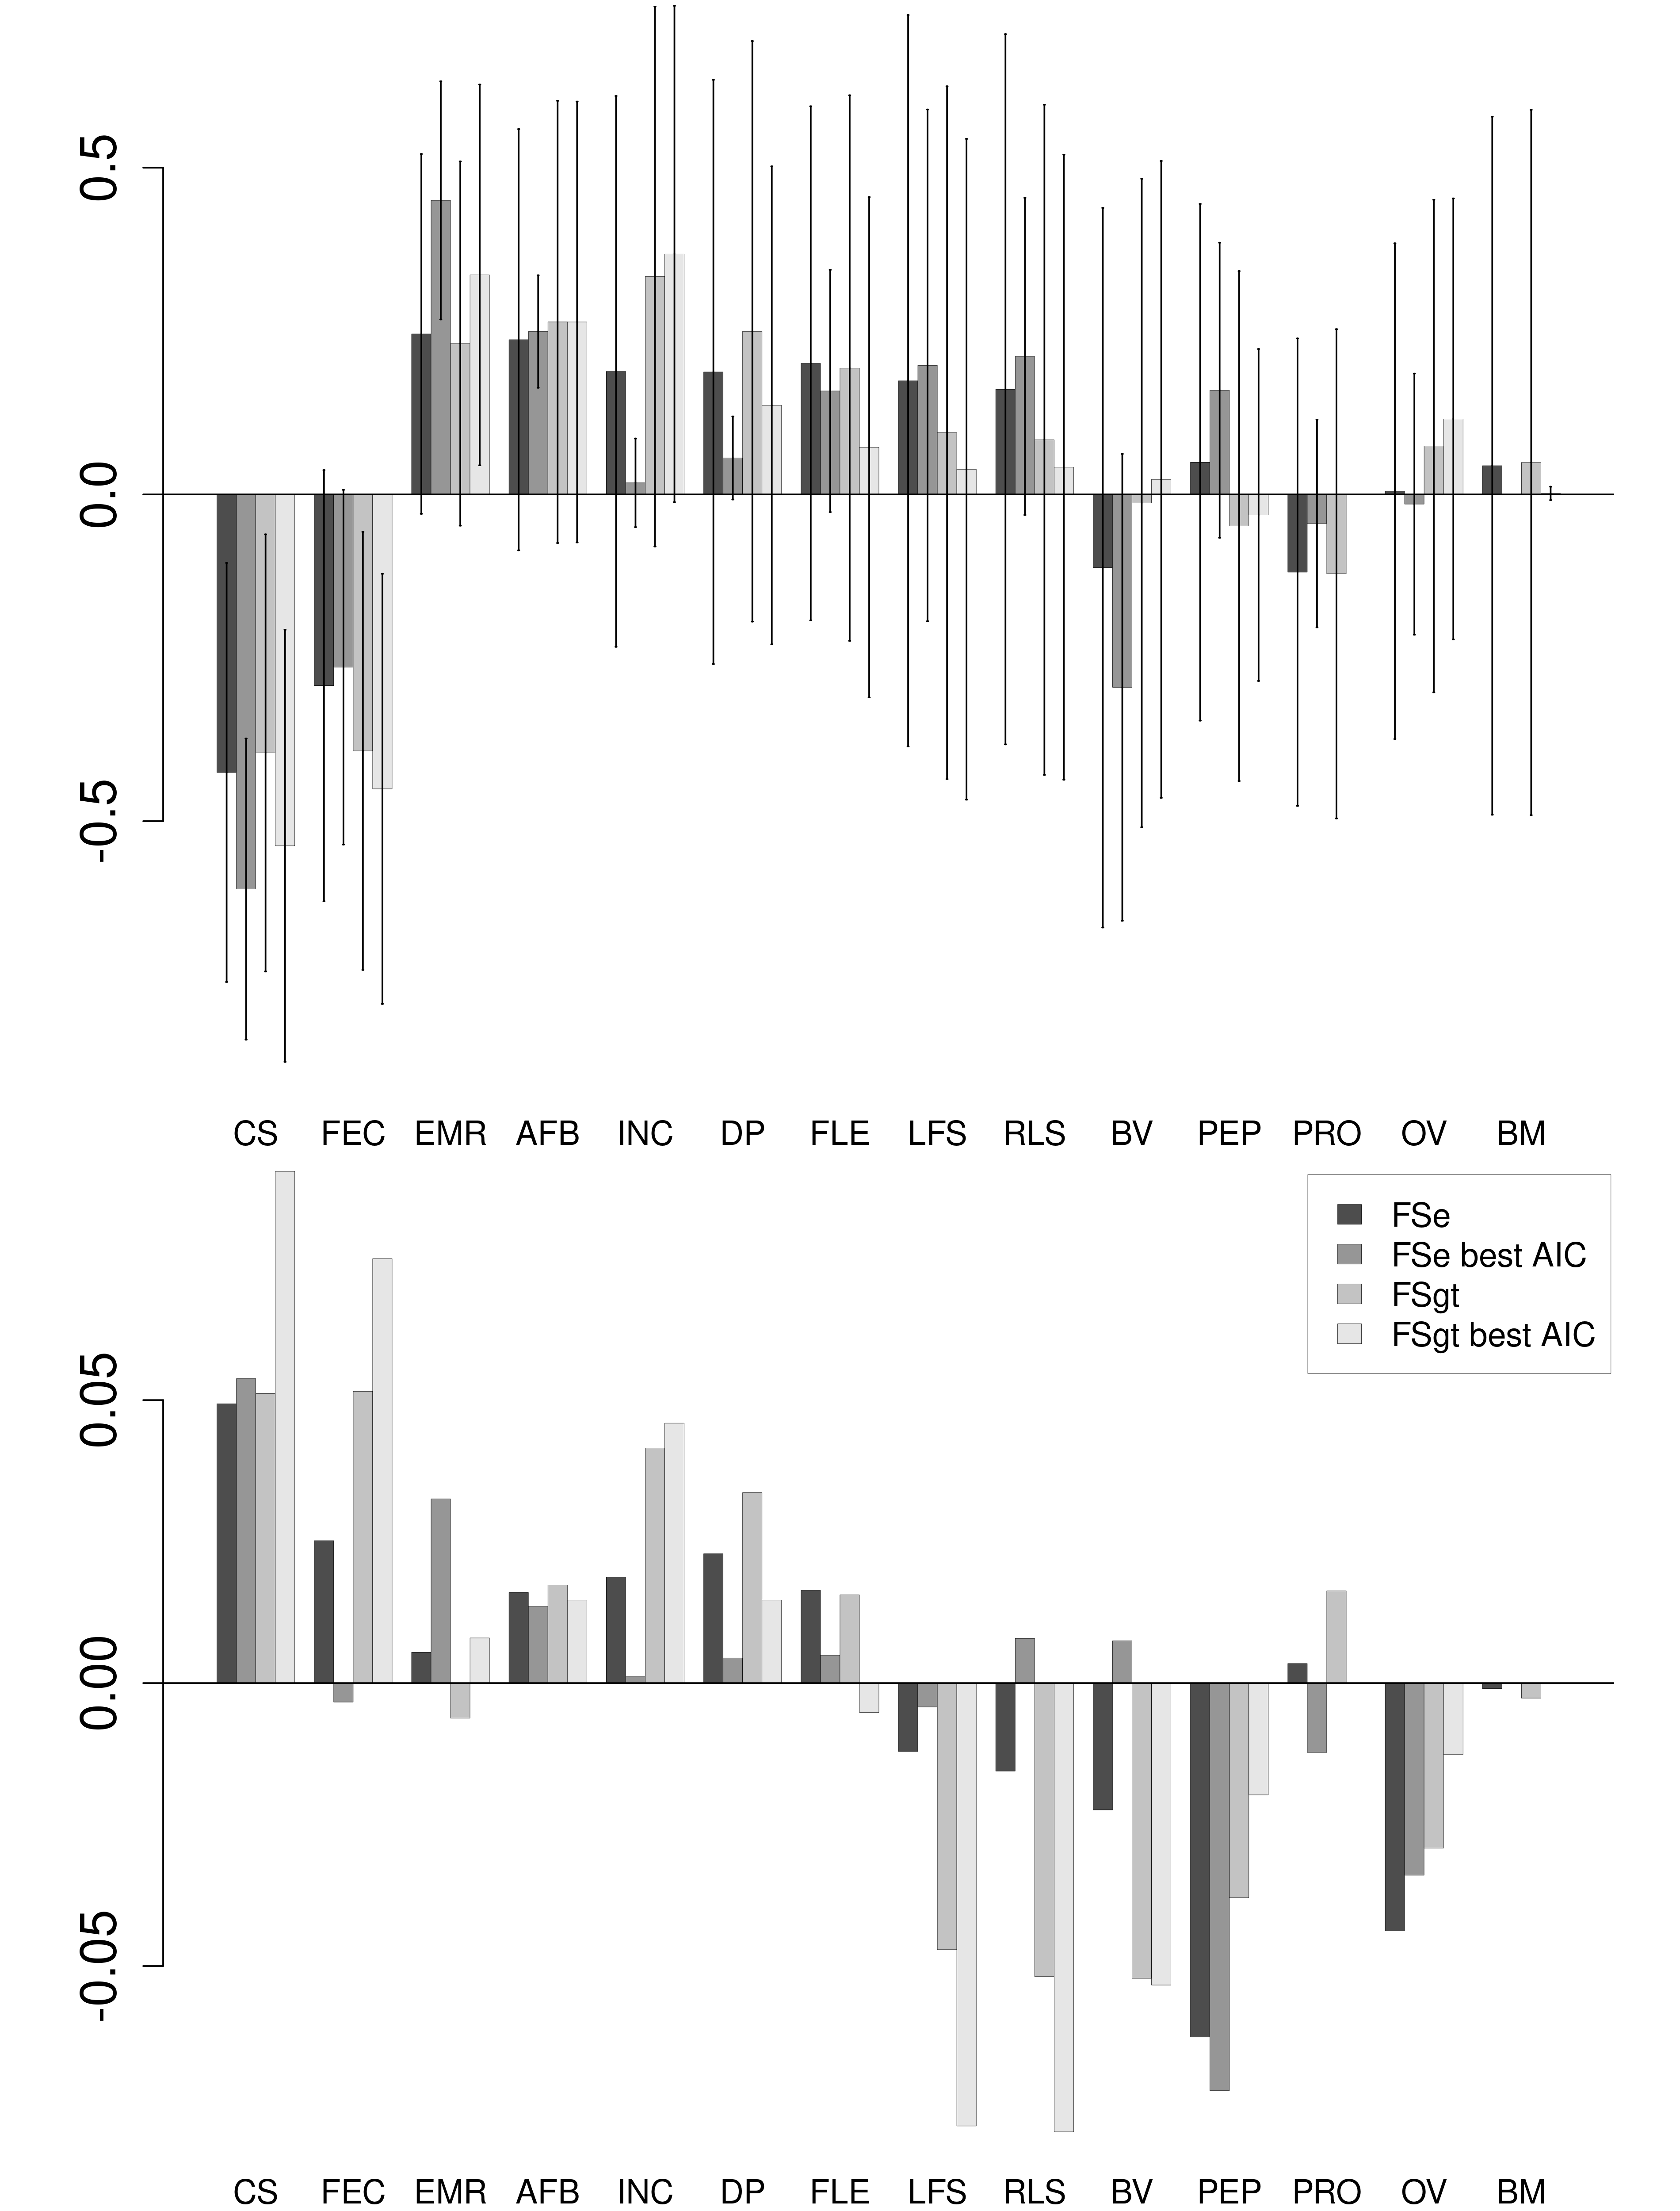
\includegraphics[width=\textwidth]{./Figures/chapter02/fig2-FSaxes.png}
\caption[Fast-Slow PC loadings]{
Importance of the traits describing the fast-slow continuum. Top panel: Loadings 
mean $\pm$ standard deviation of the selected PCs combining sets of life history
traits that better describe the fast-slow axis. Bottom panel: Relative weight
of the life history traits in the fast-slow continuum. Values range from -1 to
1, where negative values means that the absolute value of the trait loadings are
lower than expected by the frequency of the trait and positive values for traits
with higher loadings than expected by the frequency of the trait in the
selected PPCAs (see main text for details). The loadings and frequencies come
from the selected PCs that better predict elasticities to the adult survival
(FSe) or generation time (FSgt), weighted by the AIC based weight of the models
taking all or only the models with $\Delta AIC < 2$ (best AIC).}
\label{fig:fig2.2}
\end{figure}


Figure \ref{fig:fig2.2} shows the loadings of each life history trait in the 
best fast-slow axes, for both elasticities and generation time. In both cases,
the life history traits with higher and consistent weights include CS and AFB.
However, there are two main differences. First, incubation period is more 
influential for the axis based on generation time than for those based on 
elasticities. Second, FEC seems more important for PCs selected to 
predict generation time. Other traits in selected PCs have huge variability 
(see SD bars in figure \ref{fig:fig2.2} and depends on whether all models or 
only the best ones ($\Delta AIC < 2$) are used to weight the PC. Other traits 
commonly included in the fast-slow axis such as LFS or BM seems unrelated to 
the demographically defined fast-slow axis defined by our methodology.

One advantage of combining all PPCA in single weighted-average axes is that it 
allows to estimate the position of a species in the fast-slow axis even when
some scores cannot be estimated due to missing data for life history traits
combined in a PPCA. We thus estimated the fast-slow continuum for up to 1516
species for each respective axis using the extended dataset where each PCA
includes all the species with data for the included traits. The results for the
extended dataset and the Ericson backbone based phylogeny doesn't change the
patterns (see tables \ref{tab:tabApp2.2}, \ref{tab:tabApp2.3} and figures
\ref{fig:figApp2.1}, \ref{fig:figApp2.2}).

\begin{figure}
\centering
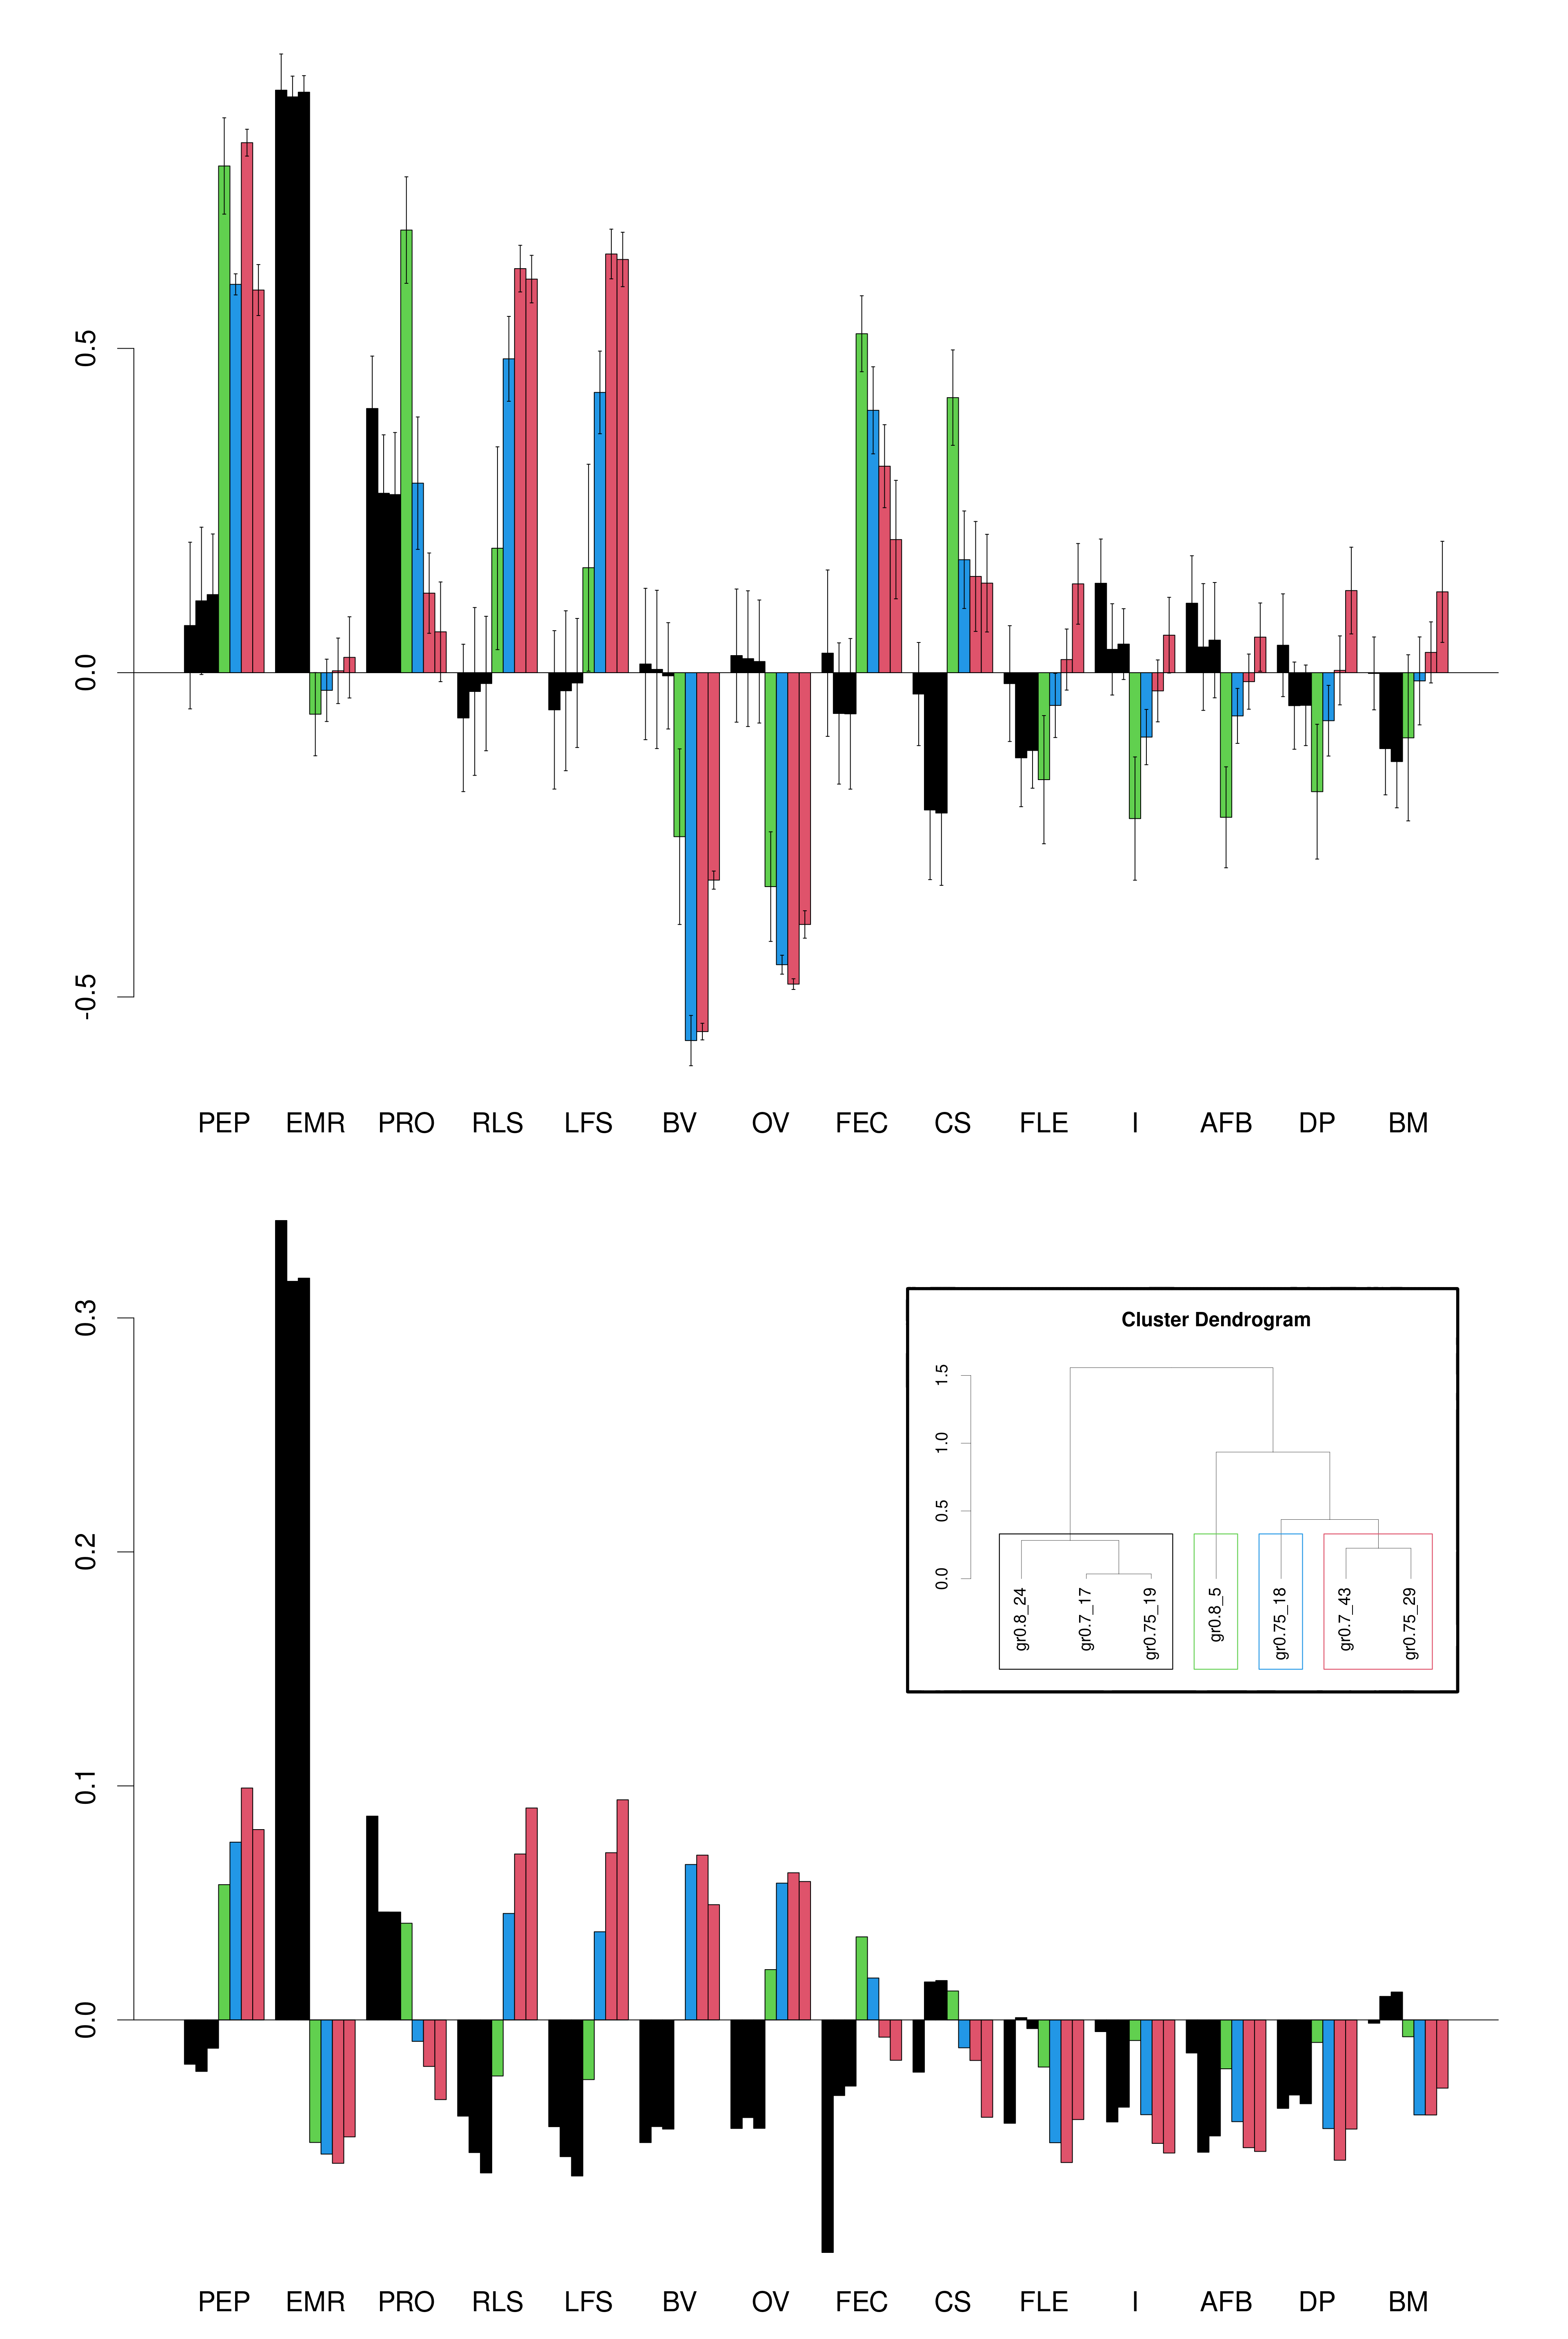
\includegraphics[width=\textwidth]{./Figures/chapter02/fig3-Secondary axes.png}
\caption[Alternative axes groups and PC loadings]{
Importance of the traits for clusters of similar significant PCs not selected
for the fast-slow axes. Each group contains PCs with scores correlation greater
than the correlation specified in the group name in the inset dendogram (e.g.
gr0.8 means correlation \textgreater{0.8}). Boxes include clusters with a
correlation among averaged loadings \textgreater{0.95} and can be conceptualized
as EMR in the black box, lifelong productivity in the green box and iteroparity
in blue and red boxes. Top panel: Loadings mean $\pm$ standard deviation for the
traits of each group of PCs. Bottom panel: Relative weight of the life history
for each group of PCs (see figure \ref{fig:fig2.2} for details).}
\label{fig:fig2.3}
\end{figure}

Although the PCs representing fast-slow continuum explains around 30\% of the
variation in life history traits ($0.35 \pm 0.07$ for FSgt, $0.34 \pm 0.06$ for
FSgt best AIC, $0.35 \pm 0.07$ for FSe and $0.29 \pm 0.05$ for FSe best AIC),
much variation still remains to be explained.
To explore this variation, we extracted all the PCs with Eigenvalue
\textgreater{1} (Kaiser-Guttman criterion) among the
%TODO: cite Kaiser criterion (Legendre P, Legendre L (2012) Numerical Ecology 
% (Elsevier, London), 3rd Ed, p 1006)
PCs not selected as descriptors of the fast-slow continuum, and classified them
in groups based on a cluster analyses of the species scores (figure
\ref{fig:fig2.3}). These clusters classify together PCs that represent similar
life history axes, which may then be interpreted by examining the loadings
of their traits.
The averaged loadings of these groups suggest at least three axes of life
history variation that are independent of the fast-slow continuum.

The most important one in terms of variance explained ($37 \pm 0.09$ \%, see
table \ref{tab:tabApp2.4} for the variance explained by each cluster, number
of traits and number of PCs) is related to the degree of iteroparity
(gr0.75\_18, gr0.7\_43 and gr0.75\_29 in figure \ref{fig:fig2.3}), quantified as
the brood value index \citep{Bokony2009}⁠, which represents whether all
reproductive effort is allocated into a few reproductive events (i.e. high brood
value as each brood has high contribution to fitness) or instead the effort is
distributed into many attempts (low brood value), whether in a same breeding
season or in different ones. Brood value is highly correlated with the RLS
(-0.89), LFS (-0.87), OV (0.92) and PEP (-0.8), thus they often appear loading
together on the same PCs.

Another life history axis that appears consistently in the analyses is related
to the offspring quality-quantity trade-off (gr0.8\_24, gr0.7\_17 and gr0.75\_19
in figure \ref{fig:fig2.3}), with species laying few eggs yet relatively large
at one extreme and species laying many eggs of small size at the other extreme.
The PCs in this group explains $0.15 \pm 0.02$ \% of the variance and the main
trait in this axis is EMR, followed by PRO and CS.

The third axes, gr0.8\_5 in figure \ref{fig:fig2.3} is related to PEP, PRO, FEC
and OV and reflects the lifelong productivity of the species in terms of
offspring number and egg mass produced relative to the body size.
% This axis is similar to the FSgt axis.
% The loadings and relative weight of OV, LFS, I, FLE AFB and BM are low
% on average but the scores of this axis are correlated with this traits
% (correlation for LFS = 0.35, I = -0.43, FLE -0.36, AFB = -0.35 and BM = -0.35).

The axes described appears consistently regardless of the phylogeny and dataset
used. See tables \ref{tab:tabApp2.5}, \ref{tab:tabApp2.6} and figures
\ref{fig:figApp2.3}, \ref{fig:figApp2.4}, \ref{fig:figApp2.5} for the details of
the extended dataset and Ericson backbone based phylogeny.

Most of the described axes exhibit high phylogenetic signal (Pagel's
$\lambda > 0.9$) except for the axes from the iteroparity group with Pagel's
$\lambda = 0.66 \pm 0.09$ and the lifelong productivity group with Pagel's
$\lambda = 0.89 \pm 0.01$ (see table \ref{tab:tabApp2.7} for details).

The two estimated fast-slow axes (FSe and FSgt) are correlated with each
other (phylogenetic correlation =  0.85 and 0.74 for all or models with
$\Delta AIC < 2$ only). Both fast-slow axes are only weakly correlated with
body mass (phylogenetic correlations = 0.34 for the axes averaging PC
scores with $\Delta AIC < 2$ and 0.5 for axes averaging all PCs). The difference
on the correlation between FSgt and FSe when includes all or only the best PCs,
suggest that BM decrease the accuracy of the PCs on predicting generation time
or the elasticity to the adult survival. In fact, there is zero PPCA containing
BM among the best models for FSe and only 3 from 487 for FSgt. The correlation
among other axes than FS, is quite low except for the lifelong productivity axis
and FSgt (-0.76) and for the lifelong productivity axis and iteroparity axes
(mean correlation $0.76 \pm 0.11$). See table \ref{tab:tabApp2.8} for detailed
correlations among axes and traits.

Scores for all described axes are available at
\href{https://github.com/jmaspons/Thesis/tree/master/ESM/chapter02}{LHT-axes.
xlsx in the ESM}.


\section{Discussion}

Our finding that not all combinations of life history traits are possible is at 
first sight unsurprising, given the existence of overwhelming evidence of life 
history trade-offs and constraints. Demonstrating it is however important 
because our empirical evidence is based on an unusually large and representative 
sample of species. We therefore can largely exclude the possibility that the 
observed pattern results from sampling biases.

The Fast-Slow continuum emerged as a major axis structuring life history 
variation in birds, confirming and generalising previous studies. Our 
empirically-derived estimates of the fast-slow continuum reflect well the 
fecundity-survival trade-off, are strongly correlated among each other and are 
largely independent of body size. Although a variety of life history traits 
contribute to define the continuum, FEC and AFB appear particularly relevant in
line with some previous suggestions. However, these life history traits are not
good surrogates of the continuum when alone, but only when combined with other
life history traits.

Many life history traits show a strong allometric relationship with adult body
mass, in part reflecting constrains associated with scaling laws. For example, 
the higher metabolic rate of smaller animals may allow them to produce offspring 
faster. However, body size may also play part on shaping the fast-slow continuum
through its effect on age-specific mortality, if for example a large body reduces
predation risk \citep{Jeschke2009}.

Although the fast-slow continuum is widely considered the most important axis of 
life history variation, growing evidence suggest the existence of other relevant 
axes. By accurately quantifying the fast-slow continuum, we could investigate 
the remaining axes of life history variation.
Our analyses identified an important axis of variation related to the timing of
reproductive bouts. This axis, the so-called brood value \citep{Bokony2009} or
semelparity-iteroparity \citep{Gaillard1989}, represents the extent to which
all reproductive effort is allocated into a few reproductive events (i.e. high
brood value) or instead the effort is distributed into many attempts (low brood
value), whether in a same breeding season or in different ones. Many species in
our dataset only breed once per year, therefore the brood value is highly
correlated with the reproductive lifespan and it often appears loading together
on the same PC. However, a low brood value may also be achieved by reproducing
multiple times during a same breeding season, a strategy that is used by some
pigeons and starlings.

Other previously suggested life history axis that appear consistently in mammals
once the fast-slow continuum is factored out is related to the duration of the
development and the trade-off between offspring quantity and quality
\citep{Promislow1990,Bielby2007,Dobson2007}. We didn't find a similar axis in
birds and it seems that this trade-off is included in our fast-slow axes, with
fast lived species investing in many and low quality offspring while slow
species invest in few but high quality offspring.

Much of the ecological relevance of the fast-slow continuum resides in its 
influence on population dynamics under challenging conditions, an issue 
particularly relevant in the current context of global environmental change. 
Species at the fast extreme have a higher potential to rapid population grow 
than those at the slow extreme, which may facilitate recovering from a 
population crash. When population size is low, however, they also tend to be 
more susceptible to populations fluctuations associated with demographic 
stochasticity. The relevance of these mechanisms can only be investigated by 
properly defining and accurately quantifying the fast-slow continuum based on 
the entire life cycle. 

Moreover, the influence of other life history axes needs also to be considered. 
A low brood value has been suggested to favour geometric population growth under 
environmental stochasticity through mechanisms such as bet-hedging 
\citep{Stearns2000a}⁠ and the storage effect \citep{Cubaynes2011}. The finding
that brood value and the fast-slow continuum are different life history axes but
share critical life history traits opens the possibility to life history
strategies that facilitate a rapid population growth when conditions are
favourable and reduce the costs of a reproductive failure when conditions are
unfavourable. For example, brood value seems a significant trait to adapt to
new environments in introduced species or species colonising urban habitats
\citep{Sol2012a,Sol2014}.

Despite having solid foundations, life history theory has surprisingly achieved 
little success in predicting the response of organisms to rapid human-induced 
environmental alterations such as habitat loss, climate change and biological 
invasions. This is paradoxical considering that some proposed mechanisms were 
proposed more than 50 years ago. A more integrative and mechanistic view of life 
history variation can contribute to develop a more predictive body of theory 
regarding how life history and the possible interactions with behaviour
\citep{Ricklefs2002,Reale2010a,Sol2018,Maspons2019} affects the response to
environmental changes. The provided axes of life history variation can open
further studies to elucidate the links between environmental condition and the
evolution of life history strategies.


\section*{Electronic Supplementary Material}

Electronic supplementary material is available online at
\url{https://github.com/jmaspons/Thesis/tree/master/ESM/chapter02}.
